\begin{tikzpicture}
\begin{axis}[width=\marginparwidth+25pt,%
tick label style={font=\scriptsize},axis y line=middle,axis x line=middle,name=myplot,axis on top,%
%			xtick={-5,-4,-3,-2,-1,1,2,3,4,5},% 
%			extra x ticks={3.14,1.57},
%			extra x tick labels={$\pi$,$\pi/2$},
%			ytick={-1,-2,1,2},
			%minor y tick num=1,%extra y ticks={-5,-3,...,7},%
%			minor x tick num=4,
			ymin=-.1,ymax=3.5,%
			xmin=-1.1,xmax=1.1%
]

\addplot [{\colorone},domain=-1:.7,smooth,thick,samples=50] {-1/(x-1)};
\addplot [{\colortwo},smooth] coordinates {(-1.,0)(-0.96,0.07686)(-0.92,0.1477)(-0.88,0.2129)(-0.84,0.2729)(-0.8,
0.328)(-0.76,0.3786)(-0.72,0.4252)(-0.68,0.468)(-0.64,0.5075)(-0.6,0.
544)(-0.56,0.578)(-0.52,0.6098)(-0.48,0.6398)(-0.44,0.6684)(-0.4,0.
696)(-0.36,0.7229)(-0.32,0.7496)(-0.28,0.7764)(-0.24,0.8038)(-0.2,0.
832)(-0.16,0.8615)(-0.12,0.8927)(-0.08,0.9259)(-0.04,0.9615)(0,1.)(0.
04,1.042)(0.08,1.087)(0.12,1.136)(0.16,1.19)(0.2,1.248)(0.24,1.311)(0.
28,1.38)(0.32,1.455)(0.36,1.536)(0.4,1.624)(0.44,1.719)(0.48,1.821)(0.
52,1.931)(0.56,2.049)(0.6,2.176)(0.64,2.312)(0.68,2.457)(0.72,2.612)(
0.76,2.777)(0.8,2.952)(0.84,3.138)(0.88,3.336)(0.92,3.545)(0.96,3.766)(1.,4.)};
%\addplot [{\colortwo!40},domain=-4:4,thick,smooth] {-x^4/2-x^3/6+x^2+x+2};

\draw (axis cs:.75,.9) node {\begin{tikzpicture}
						\draw[thick,{\colorone}] (0,0)--(10pt,0) node [right,black] {\scriptsize $\ds y= \frac{1}{1-x}$};
						\draw[{\colortwo}] (0,-15pt)--(10pt,-15pt) node [right,black] {\scriptsize $y= p_3(x)$};
													\end{tikzpicture}};
%\draw (axis cs:-2,-2.75) node {\scriptsize $y=p_{13}(x)$};



\end{axis}

\node [right] at (myplot.right of origin) {\scriptsize $x$};
\node [above] at (myplot.above origin) {\scriptsize $y$};
%\node [below] at (myplot.below origin) {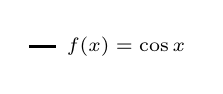
\begin{tikzpicture} \draw[thick,{\colorone}] (0,0)--(10pt,0) node [right,black] {\scriptsize $f(x)= \cos x$};\end{tikzpicture}};

\end{tikzpicture}




